\chapter{System Architecture and Design}
\label{ch:architecture}

This chapter presents the architecture of Antares AI, a privacy-preserving LLM orchestration system for enterprise workforce management. Chapter~\ref{ch:introduction} and Chapter~\ref{ch:background} set out the problem this architecture answers: an LLM has to route natural-language workforce requests without ever seeing the personal data those requests refer to. The design that follows is organised around one central invariant, no personally identifiable information crosses the LLM context boundary in cleartext, and most of the decisions described in this chapter follow from what it takes to hold that invariant in practice. Section~\ref{sec:arch_privacy_by_design} sets out the privacy-by-design principles that govern every subsequent decision. Section~\ref{sec:arch_antares_ecosystem} introduces the Antares/Miorelli domain and the constraints it places on the system. Section~\ref{sec:arch_requirements} translates those constraints into a traceable list of functional and non-functional requirements. Section~\ref{sec:arch_high_level} presents the four-service runtime architecture. Section~\ref{sec:arch_components} details the design of each component. Section~\ref{sec:arch_data_flow} traces a complete request through the system end to end.

% ==========================================
\section{Architectural Principles: Privacy-by-Design}
\label{sec:arch_privacy_by_design}

Privacy by design, formalised by Cavoukian~\cite{cavoukian2009privacy} and later codified as a legal obligation in GDPR Article~25~\cite{gdpr2016}, is the principle that privacy protection must be built into systems from the outset. Cavoukian's framework identifies seven foundational principles: proactive prevention of privacy harms, privacy as the default operational setting, privacy functionality embedded into the architecture, full functionality without zero-sum trade-offs, end-to-end security across the data lifecycle, visibility and transparency in system operation, and user-centric design. The Antares AI architecture applies these principles as structural design constraints, not as runtime policy.

Three of Cavoukian's principles shape the system most directly.

\textbf{Privacy as the default.} Anonymisation of user requests before LLM transmission is the only supported operational path. A client that skips the anonymisation step sends an unprocessed prompt, but the server system prompt still instructs the model to treat input as pseudonymised tokens; bypassing anonymisation is detectable and requires an explicit decision, not an oversight. Nothing in the system's configuration surface offers a way to switch privacy enforcement off.

\textbf{Privacy embedded into design.} PII isolation is not achieved through audit logging, access controls, or post-hoc output redaction. It is structural: by placing the anonymisation service at the architectural boundary, PII is physically absent from the data that crosses it, so there is nothing for the model to leak in the first place.

\textbf{End-to-end security.} The token-to-entity mapping is stored in an ephemeral, session-scoped Redis context and consumed exactly once during server-side deanonymisation. No component persists PII beyond the minimum lifetime required for a single business operation. Operational reports written to disk by the \texttt{JobTools} layer stay on server-local storage and are never sent to the client.

Together these constraints define the \emph{architectural invariant}: PII may exist in the system, but only within the server's trusted execution boundary, and only for the duration of one business operation.

% ==========================================
\section{The Antares AI Ecosystem}
\label{sec:arch_antares_ecosystem}

Antares AI was developed within the Antares/Miorelli ecosystem, an ERP platform for workforce management used in the Italian facility management sector. The platform manages personnel assignments to job sites (\emph{cantieri}), tracks absence and leave requests, and maintains the hierarchical relationships between workers and managers. Users currently interact via structured web interfaces; Antares AI enables the same operations through natural language, routing each request to the correct business tool automatically.

The domain is demanding on privacy and correctness for concrete reasons. The data is personnel-sensitive by nature: names, phone numbers, residential coordinates, absence records, and employment relationships are all PII under the GDPR. The user base is multilingual (requests arrive in Italian, regional dialects, or a mix), which ruled out recogniser-based NER tools designed for English. Most critically, the operational context requires accurate results: a holiday request analysis that produces an incomplete result is operationally harmful, not just inconvenient, because it may leave a client site under-staffed. The system must preserve full business logic accuracy even when anonymising inputs.

Workforce operations are structured around three core entity types: \emph{persone} (workers), \emph{cantieri} (client sites), and \emph{ticket} (absence and leave records). Relations are typed: \texttt{PULITO\_DA} links a worker to their assigned sites, \texttt{RESPONSABILE\_DI\_RIFERIMENTO} identifies a worker's manager, and \texttt{AUTORIZZATORE} identifies the person authorised to approve leave. These entity types and relation names appear in natural language requests and define the PII surface the anonymisation pipeline must cover.

% ==========================================
\section{Functional and Non-Functional Requirements}
\label{sec:arch_requirements}

The principles and domain constraints introduced above translate into a concrete set of requirements the architecture must satisfy. This section makes them explicit and traceable, without repeating the discussion already given in Sections~\ref{sec:arch_privacy_by_design} and~\ref{sec:arch_antares_ecosystem}.

\textbf{Functional requirements} follow directly from the three use cases the system supports, each one a concrete operation a dispatcher or site manager already performs by hand. Given a named client site, the architecture has to find the nearest available workers within a configurable radius and rank them by distance (Use Case~A, traced in detail in Section~\ref{sec:arch_data_flow}). Given a worker's name, it has to identify that worker's direct colleagues and surface a ranked pool of nearby substitutes (Use Case~B, Section~\ref{subsec:impl_ucb}). Given a holiday request, it has to resolve the full chain end to end: verify the requester's authorisation, determine which colleagues are absent on the relevant dates, and identify who is available to cover (Use Case~C, Section~\ref{subsec:impl_ucc}).

\textbf{Non-functional requirements} follow from the domain constraints described in Section~\ref{sec:arch_antares_ecosystem}, and each one is really a boundary condition on the functional requirements above rather than an independent property. The privacy invariant from Section~\ref{sec:arch_privacy_by_design} sets the hard limit: no PII may cross the LLM context boundary in cleartext, under any request pattern. Operational accuracy sets a second one, in the opposite direction, since a routing or entity-resolution error introduced by the privacy layer is not an acceptable trade-off when an incomplete result can leave a client site under-staffed. Multilingual support is the third: the system has to handle Italian as a native language, not as an adaptation of an English-first pipeline, given how the actual user base writes.

% ==========================================
\section{High-Level System Architecture}
\label{sec:arch_high_level}

Antares AI comprises four cooperating runtime services, each with a distinct responsibility and a well-defined interface. Figure~\ref{fig:runtime_flow} illustrates the runtime topology and data flows.

\begin{figure}[htbp]
    \centering
    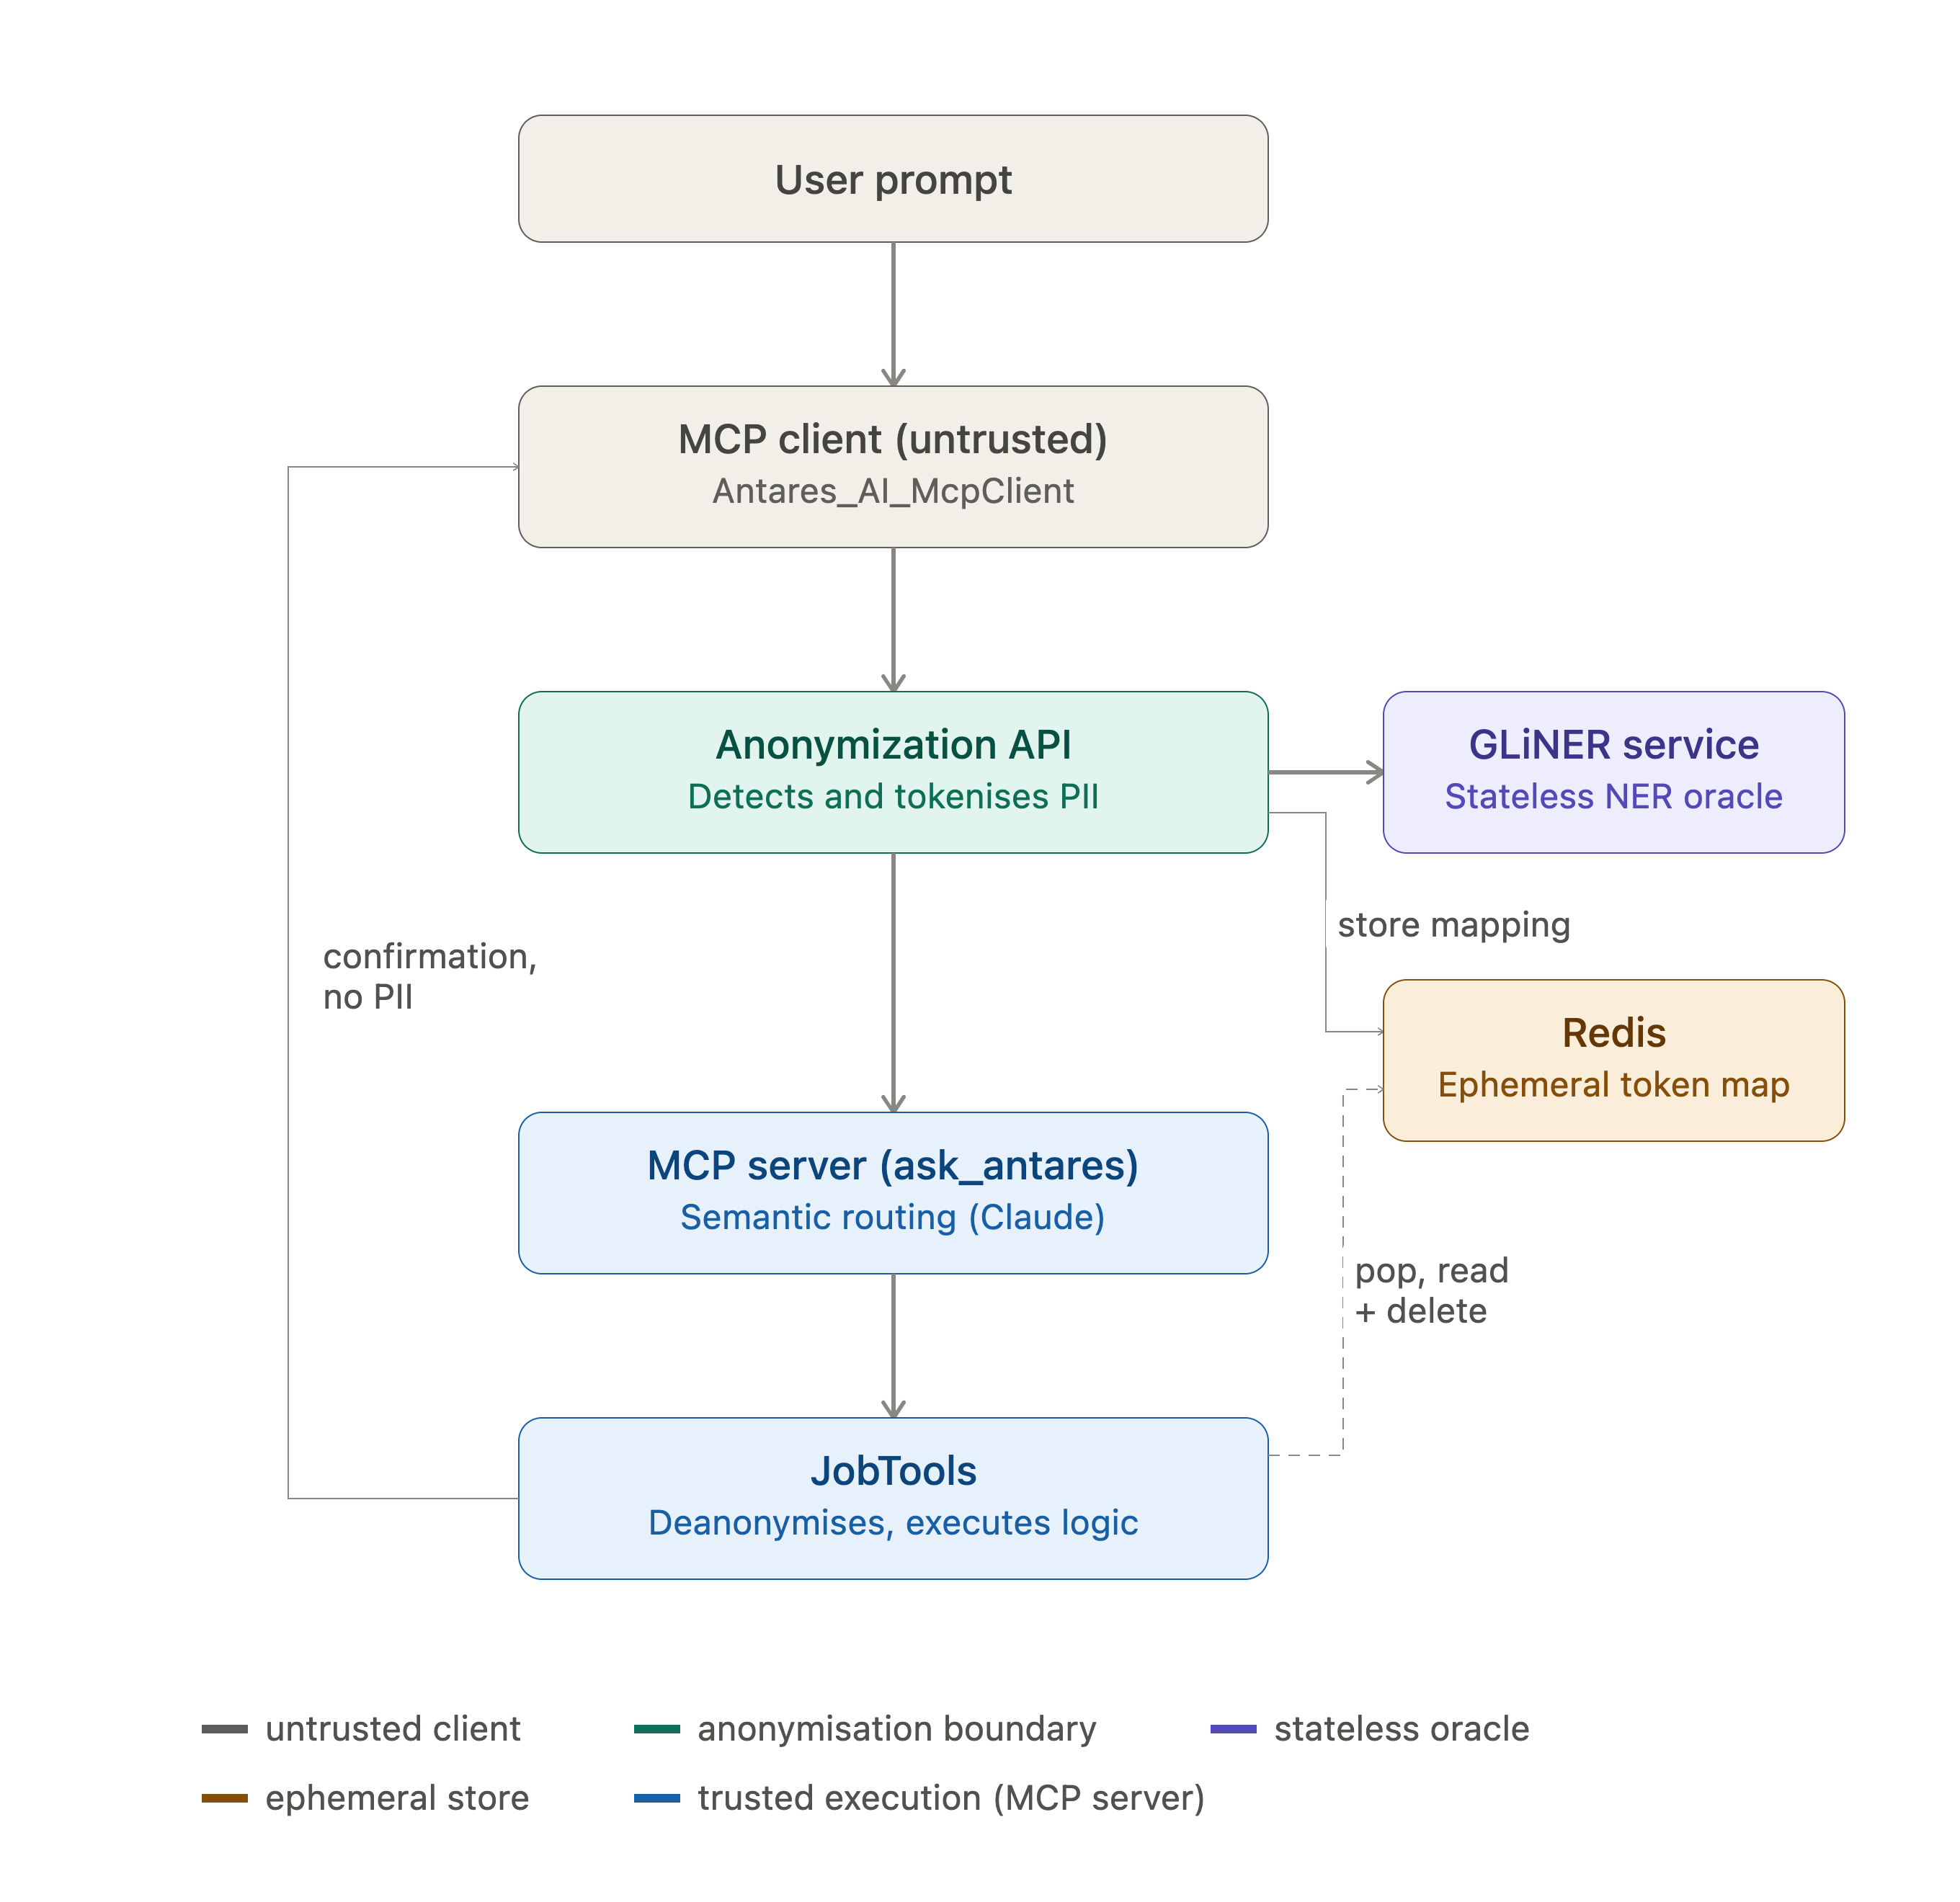
\includegraphics[width=\textwidth]{Immagini/antares_ai_secure_flow_corrected}
    \caption{Runtime architecture of Antares AI. The client anonymises the user prompt before crossing the MCP boundary. The MCP server routes the anonymised request via Claude and executes the selected business tool server-side, where PII is restored from the Redis context. The client receives only a hardcoded confirmation string.}
    \label{fig:runtime_flow}
\end{figure}

The four services and their roles are summarised in Table~\ref{tab:services}.

\begin{table}[htbp]
\centering
\caption{Antares AI runtime services}
\label{tab:services}
\begin{tabular}{llll}
\hline
\textbf{Service} & \textbf{Stack} & \textbf{Port} & \textbf{Role} \\
\hline
MCP Client & C\#/.NET~10 & --- & Request orchestration and test harness \\
Anonymization API & C\#/.NET~10 & 5292 & PII detection, tokenisation, context storage \\
GLiNER Service & Python/FastAPI & 5100 & Named entity recognition \\
MCP Server & C\#/.NET~10 & 5001 & LLM routing and business tool execution \\
\hline
\end{tabular}
\end{table}

The communication topology mirrors the system's trust model. The MCP client is an untrusted endpoint: it never receives real personnel data, and the only thing it sees is a hardcoded Italian confirmation string. The anonymisation API sits at the client-side boundary, processing the raw prompt and issuing a session token (\texttt{contextId}) that indexes the stored mapping. The GLiNER service is a stateless NER oracle; it knows nothing about tokens, Redis, or business context. The MCP server is the trusted execution boundary: it receives only anonymised prompts, routes them via Claude, restores PII server-side, and executes business tools against real data.

Redis~\cite{redis2009} runs at port~55000 as the ephemeral context store. It is not reachable from the client and is accessible only to the anonymisation API (writing) and the MCP server (reading and consuming).

The architectural invariant (no PII crosses the MCP boundary) is enforced at the interface between client and server. The \texttt{ask\_antares} tool accepts an anonymised prompt and a \texttt{contextId}; it never receives raw PII. The client calls the anonymisation API first, gets an anonymised prompt and a \texttt{contextId}, and only then constructs the tool call. PII restoration from the \texttt{contextId} happens inside the server's trusted boundary, after the routing decision has been made.

% ==========================================
\section{Component Design}
\label{sec:arch_components}

\subsection{The MCP Client Orchestrator}
\label{subsec:arch_mcp_client_orchestrator}

The MCP client (\texttt{Antares\_AI\_McpClient}) is a .NET~10~\cite{dotnet10} console application that orchestrates the end-to-end request lifecycle. In the current system it serves as both the reference client implementation and the integration test harness for the three use case scenarios.

Its responsibilities are deliberately minimal. It constructs a natural language prompt, submits it to the Anonymization API, and then calls \texttt{ask\_antares} on the MCP server with the anonymised prompt and \texttt{contextId}. The client performs no business logic and holds no sensitive data; it can't observe PII because it never calls a deanonymisation endpoint or touches the Redis context.

Communication with the MCP server uses the HTTP/SSE transport via \texttt{ModelContextProtocol.Core}. Communication with the Anonymization API uses a strongly typed HTTP client generated by NSwag~\cite{nswag2015} from the API's OpenAPI specification, keeping the client's view of the API interface in sync with the server implementation automatically.

A production client would accept dynamic user input, manage multi-turn context across \texttt{contextId} sessions, and surface token placeholders in the UI as opaque references. The current implementation uses hardcoded prompts to enable deterministic integration testing.

\subsection{The Anonymization Service API}
\label{subsec:arch_anonymization_service}

The Anonymization Service (\texttt{AnonymizationServiceAPI}) is an ASP.NET Core Minimal API application that acts as the PII gateway between client and server. It exposes three REST endpoints: \texttt{GET /anonymize}, \texttt{POST /anonymize-into-context}, and \texttt{POST /deanonymize-known}.

The primary client-facing operation is \texttt{/anonymize}. It receives a raw prompt, delegates entity detection to the GLiNER service, replaces detected entities with stable typed tokens, generates a \texttt{contextId}, stores the token-to-entity mapping in Redis, and returns the anonymised text, the \texttt{contextId}, and a detection count. The token format is \texttt{<LABEL\_NNNN>}, where \texttt{LABEL} is the uppercase entity type and \texttt{NNNN} is a zero-padded counter per label per context. This preserves entity type and cardinality while stripping identifying content.

The \texttt{/anonymize-into-context} endpoint extends an existing session by merging new token mappings into an already-issued \texttt{contextId}. This supports multi-turn interactions where a follow-up request introduces a new entity that must be pseudonymised within the same operational context.

The \texttt{/deanonymize-known} endpoint is the server-facing operation. It receives an anonymised string and a \texttt{contextId}, retrieves the mapping from Redis via a \texttt{Pop} operation (atomic read-and-delete), and restores original values through string substitution. The one-time-use design limits the exposure window for the mapping to the minimum needed for tool execution; a repeated call with the same \texttt{contextId} will find no context and fail cleanly.

Detection is fully delegated to the GLiNER service. The separation between detection (GLiNER) and masking plus context management (Anonymization API) preserves substitutability: the NER backend can be replaced without touching the tokenisation logic.

\subsection{The GLiNER-based NER Microservice}
\label{subsec:arch_gliner_ner}

The GLiNER service (\texttt{GLiNERService}) is a Python FastAPI~\cite{fastapi2018} application that exposes a single stateless endpoint, \texttt{POST /analyze}, and a health check at \texttt{GET /health}. Its job is to apply the GLiNER model to an input text and return a list of detected entity spans with labels, character offsets, and confidence scores.

The multilingual model \texttt{urchade/gliner\_multi-v2.1}~\cite{zaratiana2023gliner} is loaded once at startup and held in memory for the process lifetime. Model weights download from HuggingFace on first run and are cached locally; subsequent starts use the cached copy.

The service is a dumb NER oracle. It receives text and labels, runs the model, returns spans. All policy decisions (which labels to request, what confidence threshold to apply, how to handle overlapping spans) are made by the Anonymization API, which configures the \texttt{/analyze} call accordingly. This keeps the GLiNER service simple and reusable.

Three post-processing stages run within the Anonymization API before token substitution. Raw predictions are normalised: invalid offsets, missing labels, and out-of-bounds spans are discarded. Low-quality entities are filtered out: spans below the 0.45 confidence threshold, spans shorter than three characters, and spans matching an Italian stopword blocklist are removed. Overlapping predictions are deduplicated, keeping the higher-confidence, longer span. The result is a clean, non-overlapping list of entity spans ready for replacement.

\subsection{The Antares MCP Server}
\label{subsec:arch_antares_mcp_server}

The MCP server (\texttt{Antares\_AI\_McpServer}) is the trusted execution boundary. It exposes the \texttt{ask\_antares} routing tool, calls the Claude API for semantic routing, and executes the selected business tool against the Miorelli data layer.

Tools are registered via \texttt{ModelContextProtocol.AspNetCore}, which generates MCP-compliant schemas from C\# class and method annotations. Two types are registered: \texttt{AntaresTools} (exposing \texttt{ask\_antares}) and \texttt{JobTools} (exposing the three business operations). The \texttt{JobTools} methods are not called directly by the MCP client; Claude invokes them through function-calling within an \texttt{ask\_antares} execution.

The server calls Claude~Sonnet~4.6 via the \texttt{Anthropic.SDK} client. The system prompt defines Claude's role as a semantic router, lists the available sub-tools with descriptions, and enforces privacy constraints: the model must not infer or reveal PII from tokens, must forward the \texttt{contextId} to the selected sub-tool, and must include the sub-tool's result string verbatim in its response. A retry loop with exponential backoff handles transient \texttt{overloaded\_error} responses, retrying up to four times before returning an error message.

The data access layer is abstracted behind \texttt{IMiorelliService}. The current implementation registers \texttt{MiorelliServiceStub}, which throws \texttt{MiorelliClientNotAvailableException} on every call; each business tool catches this and falls back to static mock data from \texttt{MiorelliMockDataProvider}. Switching to the real Miorelli tenant requires changing one line in \texttt{program.cs}: registering \texttt{AntaresMiorelliClient} instead of the stub. No tool code changes. This design is discussed in Chapter~\ref{ch:implementation}.

% ==========================================
\section{Data Flow and Lifecycle of a Request}
\label{sec:arch_data_flow}

This section traces a user request from natural language prompt to confirmation response. Use Case~A (finding the nearest available workers to a named client site) serves as the concrete example.

\subsection{Tokenisation and Ephemeral Context Storage}
\label{subsec:arch_tokenization_redis}

The lifecycle begins when the MCP client constructs a natural language prompt. For Use~Case~A, a typical prompt is: \emph{``Trova i lavoratori più vicini al cantiere Bergamo Via della Fonda~5 Giulia S.r.l.\ entro~15~km. Risolvi tutti i GUID internamente.''} This contains two PII spans: a location name (\emph{Bergamo Via della Fonda~5}) and a company name (\emph{Giulia S.r.l.}).

The client calls \texttt{GET /anonymize}. The API calls the GLiNER service, receives entity predictions, runs the three-stage filtering pipeline, and sorts surviving entities by character offset in reverse order. Replacements are applied right-to-left to avoid invalidating offsets of earlier spans. The location becomes \texttt{<LOCATION\_0001>} and the company becomes \texttt{<ORGANIZATION\_0001>}.

The mapping \texttt{\{"<LOCATION\_0001>": "Bergamo Via della Fonda 5", "<ORGANIZATION\_0001>": "Giulia S.r.l."\}} is stored in Redis under \texttt{anon:context:\{contextId\}}, where \texttt{contextId} is a freshly generated UUID. The API returns the anonymised prompt and the \texttt{contextId} to the client. No PII is in the response; the client holds only an opaque session identifier.

Redis is the right tool here for practical reasons: its in-memory architecture gives sub-millisecond read and write latency, which matters in a synchronous request pipeline. Its native hash type matches the token-map structure directly, and its in-memory-with-optional-persistence model suits ephemeral session data that does not need to survive a service restart.

\subsection{Isolated Semantic Routing}
\label{subsec:arch_semantic_routing}

The client constructs the \texttt{ask\_antares} tool call with the anonymised prompt and \texttt{contextId}, dispatching it over HTTP/SSE. At this point the MCP boundary has been crossed and no PII is in transit.

The \texttt{ask\_antares} implementation builds a Claude API call. The system prompt defines Claude's role as an Italian-language semantic router, provides the JSON schemas of the available sub-tools, and specifies the expected response format. The anonymised user prompt becomes the user message.

Claude's task is intent classification (which sub-tool?) and parameter extraction (what values, in anonymised form?). For Use~Case~A it classifies the intent as \texttt{get\_nearest\_workers\_to\_cantiere} and extracts \texttt{cantiereName = "<LOCATION\_0001>"} and \texttt{context\_id = \{contextId\}}. It doesn't try to resolve the token; it works entirely with the pseudonymised representation.

The Claude API returns a structured tool call rather than free text. The \texttt{Microsoft.Extensions.AI} abstraction intercepts it, locates the registered \texttt{GetNearestWorkersToCantiere} method, and invokes it with the extracted parameters. The Redis context is not touched during this phase.

\subsection{Server-Side Deanonymisation and Tool Execution}
\label{subsec:arch_deanonymization}

The \texttt{GetNearestWorkersToCantiere} method is the first point where PII re-enters the system. Its first action is to call \texttt{DeanonymizeAsync}, which posts to \texttt{/deanonymize-known} with the token \texttt{"<LOCATION\_0001>"} and the \texttt{contextId}. The API atomically reads and deletes the context from Redis and returns the original value: \texttt{"Bergamo Via della Fonda 5"}. The Redis context no longer exists after this call.

The deanonymised value drives the business logic entirely within the server's trusted boundary. The method resolves the caller's authorised cantieri via the Miorelli service layer, locates the matching site, retrieves assigned workers via the \texttt{PULITO\_DA} relation, computes Haversine distances from each worker's registered coordinates to the site's GPS coordinates, and filters and ranks results by distance within the specified radius.

The full report, containing real names, phone numbers, distances, and status information, is written to a timestamped file in the server's local \texttt{logs/} directory. It is never transmitted to the client. The method returns a hardcoded Italian confirmation string: \emph{``Operazione completata con successo.''} Claude includes this verbatim in its final response.

The client receives a short text block with no PII. The invariant holds across the entire lifecycle: no personally identifiable information crossed the MCP boundary, and a complete, accurate operational result was produced server-side.
